\section{System overview}

Heart of SoC is CPU. The CPU is only one master on the system bus and it control
all communication on this bus. To the CPU is directly connected interrupt
controller.

Bus consist of 24b address, 32b MOSI data, 32b MISO data, clock, reset, write,
read and ack signals. There is also 32b bus for interrupts.

All the peripherals are connected to the system bus, CPU select peripheral to
communicate with through address. Peripheral control ack signal to say to CPU
"data is ready for read" when CPU want read data, or "data is written" when CPU
want write data. This allow slower peripheral to cooperate with CPU, CPU simply
wait for them.

Some peripherals have special pins, these are commonly connected to the top
level entity pins, but there are few that are connected internally, for example
pll outputs.

CPU have multiple clock domain. At this moment there are two domains, one is for
VGA pixel clock and another is for rest SoC (CPU/Timers/UARTs and so on).
Clocks are generated by pll from 50MHz input. 50MHz was selected because 50MHz
oscillators are common on the Terasic FPGA boards.

\begin{wrapfigure}{L}{0.6\textwidth}
    \centering
    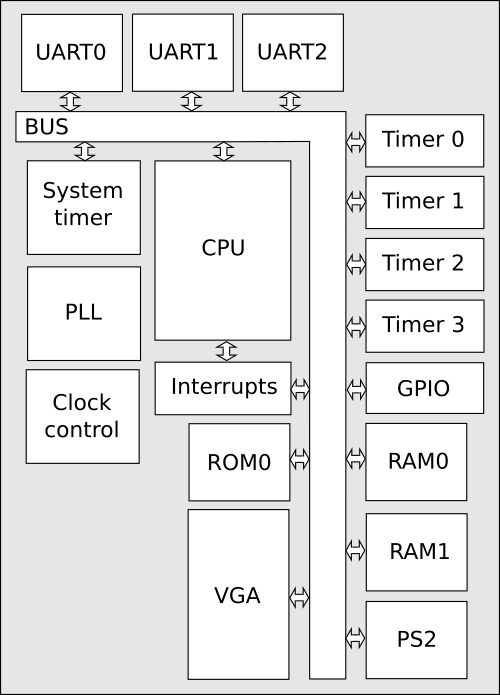
\includegraphics[width=0.55\textwidth]{img/MARK_II.png}
    \caption{MARK-II system architecture}
    \label{fig:sysarch}
\end{wrapfigure}

On the figure \ref{fig:sysarch} is simple high level schematic of MARK-II system architecture,
you can see bus, CPU and all units. PLL and clock control are only two units
that are not connected to the main BUS. They are don't need any configuration.

PLL unit is generating predefined frequencies, and clock control unit is
generating control signals for clock dividers in other modules.

Another special module is interrupt control unit. It is connected directly to
the CPU and also connected on system BUS. Interrupt control unit have interrupt
sources that are connected to the others modules such are Timers or UARTs.

\subsection{Memory map}

\begin{table}[]
    \centering
    \begin{tabular}{|l|l|l|l|l|}
        \hline
        \textbf{Peripheral} & \textbf{Base} & \textbf{Size} & \textbf{End} & \textbf{Note}                                  \\ \hline
        ROM                 & 0x000000      & $2^{8}$       & 0x0000FF     & Read only memory                               \\ \hline
        GPIO                & 0x000100      & $2^{2}$       & 0x000103     & General purpose inputs and outputs             \\ \hline
        System Timer        & 0x000104      & $2^{1}$       & 0x000105     & 24b system timer                               \\ \hline
        Interrupt driver    & 0x000108      & $2^{0}$       & 0x000108     & Enable and disable interrupts                  \\ \hline
        PS2 Keyboard        & 0x000109      & $2^{0}$       & 0x000109     & PS2 interface driver                           \\ \hline
        UART 0              & 0x00010A      & $2^{1}$       & 0x00010B     & Serial port 0                                  \\ \hline
        UART 1              & 0x00010C      & $2^{1}$       & 0x00010D     & Serial port 1                                  \\ \hline
        UART 2              & 0x00010E      & $2^{1}$       & 0x00010F     & Serial port 2                                  \\ \hline
        Timer 0             & 0x000110      & $2^{2}$       & 0x000113     & General purpose timer 0                        \\ \hline
        Timer 1             & 0x000114      & $2^{2}$       & 0x000117     & General purpose timer 1                        \\ \hline
        Timer 2             & 0x000118      & $2^{2}$       & 0x00011B     & General purpose timer 2                        \\ \hline
        Timer 3             & 0x00011C      & $2^{2}$       & 0x00011F     & General purpose timer 3                        \\ \hline
        on-chip RAM0        & 0x000400      & $2^{10}$      & 0x0007FF     & Simple onchip RAM - fastest RAM in SoC         \\ \hline
        VGA                 & 0x001000      & $2^{13}$      & 0x001FFF     & VGA GPU - text mode output 80x30 chars         \\ \hline
        on-chip RAM1        & 0x100000      & $2^{13}$      & 0x101FFF     & Simple onchip RAM - fastest RAM in SoC         \\ \hline
    \end{tabular}
    \caption{Memory map}
    \label{tab:memory_map}
\end{table}

In the table \ref{tab:memory_map} is simple memory map. There are listed all
peripherals implemented in MARK II SoC. Each peripheral have one or more registers at different
addresses.

Lets say, GPIO have 0x00100 as base address, one of the GPIO register
is DDRB register with offset +3, so address of DDRB register is 0x00103. For
informations about individual register please see corresponding peripheral sections.

\subsection{Interrupt sources}

\begin{table}[]
    \centering
    \begin{tabular}{|l|l|l|l|}
        \hline
        \textbf{Int number} & \textbf{Peripheral} & \textbf{Vector} & \textbf{Purpose}               \\ \hline
        0                   & System Timer        & 0x000010        & Timer compare match / overflow \\ \hline
        1                   & -                   & 0x000012        & -                              \\ \hline
        2                   & -                   & 0x000014        & -                              \\ \hline
        3                   & -                   & 0x000016        & -                              \\ \hline
        4                   & -                   & 0x000018        & -                              \\ \hline
        5                   & -                   & 0x00001A        & -                              \\ \hline
        6                   & -                   & 0x00001C        & -                              \\ \hline
        7                   & -                   & 0x00001E        & -                              \\ \hline
        8                   & UART0               & 0x000020        & Byte sended                    \\ \hline
        9                   & UART0 Rx            & 0x000022        & Byte recieved                  \\ \hline
        10                  & UART1 Tx            & 0x000024        & Byte sended                    \\ \hline
        11                  & UART1 Rx            & 0x000026        & Byte recieved                  \\ \hline
        12                  & UART2 Tx            & 0x000028        & Byte sended                    \\ \hline
        13                  & UART2 Rx            & 0x00002A        & Byte recieved                  \\ \hline
        14                  & Timer 0             & 0x00002C        & Timer compare match / overflow \\ \hline
        15                  & Timer 1             & 0x00002E        & Timer compare match / overflow \\ \hline
        16                  & Timer 2             & 0x000030        & Timer compare match / overflow \\ \hline
        17                  & Timer 3             & 0x000032        & Timer compare match / overflow \\ \hline
        18                  & PS2 Keyboard        & 0x000034        & Byte recieved                  \\ \hline
        19                  & -                   & 0x000036        & -                              \\ \hline
        20                  & -                   & 0x000038        & -                              \\ \hline
        21                  & -                   & 0x00003A        & -                              \\ \hline
        22                  & -                   & 0x00003C        & -                              \\ \hline
        23                  & -                   & 0x00003E        & -                              \\ \hline
        24                  & -                   & 0x000040        & -                              \\ \hline
        25                  & -                   & 0x000042        & -                              \\ \hline
        26                  & -                   & 0x000044        & -                              \\ \hline
        27                  & -                   & 0x000046        & -                              \\ \hline
        28                  & -                   & 0x000048        & -                              \\ \hline
        29                  & -                   & 0x00004A        & -                              \\ \hline
        30                  & -                   & 0x00004C        & -                              \\ \hline
        31                  & -                   & 0x00004E        & -                              \\ \hline
    \end{tabular}
    \caption{List of all interrupt sources}
    \label{tab:intsources}
\end{table}

In the table \ref{tab:intsources} are listed all interrupt vectors. Destinations
adresses of interrupts are hardwired into CPU and cannot be changed. All
interrupts are mascable using interrupt controller.

Support for nested interrupts isn't implemented. When one interrupt come, CPU
will jump into interrupt service routine and until RETI instruction is executed,
another interrupt cannot be raised. Anyway, when an interrupt is active, another
one is then put into queue.

\subsection{Brief peripheral informations}

\subsubsection{On-chip ROM}

On-chip ROM is small memory for your program, it can be initialized with content
 at the synthesizing design into FPGA. This memory have only 1kB (256 words).

\subsubsection{GPIO}

Really simple peripheral but widely used. GPIO consist from two eight bit ports.
 Each pin in port can be configured as output or input.

\subsubsection{SysTimer}

Simple 24b timer. It will generate interrupt on compare match and then start
counting from zero.

\subsubsection{Interrupt driver}

Simple interrupt controller allowing disabling individual interrupts. Also take
care about priorities.

\subsubsection{UART}

Universal asynchronous receiver/transmitter is intended for serial comunication
with many devices like computers, another microcontrollers, modules and so on.
It has build in baud rate generator and also generate interrupts when byte is
received or transmitted.

\subsubsection{Timers}

Basic 16b timers with PWM output generation and interrupts. Timer can generate
interrupt on compare match like SysTimer, on overflow or on both.

\subsubsection{On-chip RAM}

Bigger place for data and program. CPU can run program from there too because
it is designed as Von Neuman architecture. RAM have 4kB in size, so there are
1024 words. This RAM is faster than external, you can use it for accelerate your
programs by storing them here, or at least, store variables here.

\subsubsection{PS2 driver}

With PS2 driver you can connect keyboard to the SoC. This driver is really
simple and it is able only to receive data from keyboard. It will also generate
interrupt when data from keyboard come.

\subsubsection{VGA driver}

VGA driver is useful form of output. It work in text mode with resolution 80x30
characters. Each character have size 8x16 pixels. This is 640x480@73hz effective
resolution. VGA driver also support colors, you can specify color for foreground
(character) and for background.
